\chapter{Angular momentum}
\section{Angular momentum }
The angular momentum of a particle about a point is defined in position vector of a particle with the given point as the origin of the co-ordinate system and $p$ is the linear momentum.\\\\
Analogically in quantum mechanics there exist quantum mechanically orbital angular momentum is defined as
\begin{align*}
L&=L_{x} \hat{i}+L_{y} \hat{j}+L_{z} \hat{k}\\
\text{where}&\\
L_{x}&=Y P_{z}-Z P_{y}\\
L_{y}&=Z P_{x}-X P_{z}\\
L_{z}&=X P_{y}-Y P_{x}\\
\intertext{where $X, Y, Z$ are position operator in $x, y, z$ direction and $p_{1}, p_{y}, p_{z}$ momentum in respective
	$x, y, z$ direction it is given that }
P_{x}&=-i \hbar \frac{\partial}{\partial x},\\
 P_{v}&=-i \hbar \frac{\partial}{\partial y}\\
P_{z}&=-i \hbar \frac{\partial}{\partial z}\\
\text{In quantum mechanics one}&\text{ can defined the Hermitian operator}\\
L^{2}&=L_{x}^{2}+L_{y}^{2}+L_{z}^{2}
\end{align*}
\subsubsection{Commutation Relation}
\begin{align*}
{\left[\hat{L}_{x}, \hat{L}_{y}\right]=i \hbar \hat{L}_{z}} & {\left[\hat{L}_{y}, \hat{L}_{z}\right]=i \hbar \hat{L}_{x}} {\left[\hat{L}_{z}, \hat{L}_{x}\right]=i \hbar \hat{L}_{y}} \\
{\left[\hat{L}_{y}, \hat{L}_{x}\right]=-i \hbar \hat{L}_{z}} & {\left[\hat{L}_{z}, \hat{L}_{y}\right]=-i \hbar \hat{L}_{x}}  {\left[\hat{L}_{x}, \hat{L}_{z}\right]=-i \hbar \hat{L}_{y}}
\end{align*}
i.e. the components of the orbital angular momentums cannot be measured simultaneously accurately.
\begin{align*}
\left[\hat{L}^{2}, \hat{L}_{x}\right]&=0\\
\left[\hat{L}^{2}, \hat{L}_{y}\right]&=0 \quad\left[\hat{L}^{2}, \hat{L}_{z}\right]=0
\end{align*}
i.e. square of the orbital angular momentum commutes with any one of components of the orbital angular momentum.
\begin{align*}
\left[\hat{L}_{x}, \hat{p}_{x}\right]&=0\\
\left[\hat{L}_{y}, \hat{p}_{y}\right]&=0 \quad\left[\hat{L}_{z}, \hat{p}_{z}\right]=0
\end{align*}
$\begin{array}{lll}
	{\left[\hat{L}_{x}, \hat{p}_{y}\right]=i \hbar \hat{p}_{z}}  & {\left[\hat{L}_{y}, \hat{p}_{z}\right]=i \hbar \hat{p}_{x}} & {\left[\hat{L}_{z}, \hat{p}_{x}\right]=i \hbar \hat{p}_{y}} \\\\
	{\left[\hat{L}_{x}, \hat{x}\right]=0} & {\left[\hat{L}_{y}, \hat{y}\right]=0} & {\left[\hat{L}_{z}, \hat{z}\right]=0} \\\\
	{\left[\hat{L}_{x}, \hat{y}\right]=i \hbar \hat{z}} & {\left[\hat{L}_{y}, \hat{z}\right]=i \hbar \hat{x}} & {\left[\hat{L}_{z}, \hat{x}\right]=i \hbar \hat{y}}
\end{array}$
\subsection{Orbital angular momentum in sperical polar coordinates }
\begin{align*}
L_{x}&=i\hbar\left(\sin \phi \frac{\partial}{\partial \theta}+\cos \phi \cot \theta \frac{\partial}{\partial \phi}\right) \\
L_{y}&=i \hbar\left(-\cos \phi \frac{\partial}{\partial \theta}+\sin \phi \cot \theta \frac{\partial}{\partial \phi}\right) \text { and }\\
L_{z}&=-i \hbar \frac{\partial}{\partial \phi}
\end{align*}
\subsection{eigen value and eigen vector of $L^2$ and $L_z$}
Since,the commutator bracket $\left[ L^2,L_z\right] =0$ therefore $L^2$ and $L_z$ can be measured simultaneously accurately and both have simultaneous eigenfunctions and eigenkets.Denoting the simultaneous eigen kets $|l,m_l\rangle $ (Where l and $m_l$ are the orbital quantum number magnetic quantum number respectevely),the eigen value equation for $L^2$ and $L_z$ can be written as 
\begin{align*}
\hat{L}^{2}\left|l, m_{l}\right\rangle&=l(l+1) \hbar^{2}\left|l, m_{l}\right\rangle \\
\hat{L}_{z}\left|l, m_{l}\right\rangle&=m_{l} \hbar\left|l, m_{l}\right\rangle\\
\text { Alternate form: Since, } \hat{L}^{2} \text { and } \hat{L}_{z} &\text { depends on } \theta, \phi \text { then their eigen function is function of } \theta, \phi \text { i.e. }\\
\hat{L}^{2} Y_{\ell, m_{l}}(\theta, \phi)&=\ell(\ell+1) \hbar^{2} Y_{\ell, m_{l}}(\theta, \phi) \\
\hat{L}_{z} Y_{\ell, m_{l}}(\theta, \phi)&=m_{l} \hbar Y_{\ell, m_{l}}(\theta, \phi)\\
\text { where } Y_{\ell, m}(\theta, \phi) \text{is said to be}&\text {  Spherical Harmonics and defined as }\\
Y_{l, m_{l}}(\theta, \varphi)&=\varepsilon \sqrt{\left(\frac{2 \ell+1}{4 \pi}\right) \frac{\left(\ell-\left|m_{l}\right|\right) !}{\left(\ell+\left|m_{l}\right|\right) !}} P_{\ell}^{\left|m_{l}\right|}(\cos \theta) e^{i m_{l} \phi}\\
\text { where } \varepsilon&=(-1)^{m_{l}} \text { for } m_{l}>0 \text { and } \varepsilon=1 \text { for } m_{l} \leq 0 \text {. }
\end{align*}
\subsection{Lowering and Raising Operators}
\begin{align*}
	\text { Raising Operator: }  \hat{L}_{+}&=\hat{L}_{x}+i \hat{L}_{y}\\
\text { Lowering Operator: }  \hat{L}_{-}&=\hat{L}_{x}-i \hat{L}_{y}
\end{align*}
\textbf{Important relations:}
$$
\begin{array}{lll}
{\left[\hat{L}_{x}, \hat{L}_{+}\right]=-\hbar \hat{L}_{z}}&{\left[\hat{L}_{x}, \hat{L}_{-}\right]=\hbar \hat{L}_{z}}\\\\
{\left[\hat{L}_{z}, \hat{L}_{+}\right]=\hbar \hat{L}_{+}} & {\left[\hat{L}_{z}, \hat{L}_{-}\right]=-\hbar \hat{L}_{-}}  \\\\
{\left[\hat{L}_{y}, \hat{L}_{+}\right]=-i \hbar \hat{L}_{z}} & {\left[\hat{L}_{y}, \hat{L}_{-}\right]=i \hbar \hat{L}_{z}} & {\left[\hat{L}_{+}, \hat{L}_{-}\right]=2 \hbar \hat{L}_{z}} \\\\
\hat{L}_{+} \hat{L}_{-}=\hat{L}^{2}-\hat{L}_{z}^{2}+\hbar \hat{L}_{z} & \hat{L}_{-} \hat{L}_{+}=\hat{L}^{2}-\hat{L}_{z}^{2}-\hbar \hat{L}_{z}
\end{array}
$$
$\text { Action of } \hat{L}_{+} \text {and } \hat{L}_{-}:$
\begin{align*}	
\hat{L}_{+}\left|l, m_{l}\right\rangle&=\sqrt{\left(\ell-m_{l}\right)\left(l+m_{l}+1\right)} \hbar\left|l, m_{l}+1\right\rangle \\
\hat{L}_{+} Y_{\ell, m_{l}}(\theta, \phi)&=\sqrt{\left(\ell-m_{l}\right)\left(l+m_{l}+1\right)} \hbar Y_{i, m_{i}+1}(\theta, \phi)\\
\hat{L}_{-}\left|l, m_{l}\right\rangle&=\sqrt{\left(\ell+m_{l}\right)\left(l-m_{l}+1\right)} \hbar\left|l, m_{l}-1\right\rangle \\
\hat{L}_{-} Y_{\left(, m_{l}\right.}(\theta, \phi)&=\sqrt{\left(\ell+m_{l}\right)\left(l-m_{l}+1\right)} \hbar Y_{\ell, m_{l}-1}(\theta, \phi)
\end{align*}
\subsection{ Matrix Representation of the operators:}
\begin{align*}
\intertext{Elements of $\hat{L}^{2}=\left\langle\ell^{\prime}, m_{l}^{\prime}\left|\hat{L}^{2}\right| \ell, m_{l}\right\rangle=\ell(\ell+1) \hbar^{2} \delta_{\ell \ell^{\prime}} \delta_{m_{l} m_{l}^{\prime}}$, will be non-zero for $l=l^{\prime}$ and $m_{l}=m_{l^{\prime}}$ is}
\hat{L}^{2}&=\left[\begin{array}{lll}
2 \hbar^{2} & 0 & 0 \\
0 & 2 \hbar^{2} & 0 \\
0 & 0 & 2 \hbar^{2}
\end{array}\right]=2 \hbar^{2}\left[\begin{array}{lll}
1 & 0 & 0 \\
0 & 1 & 0 \\
0 & 0 & 1
\end{array}\right](\text { for } l=1)
\intertext{Elements of $\hat{L}_{z}=\left\langle\ell^{\prime}, m_{l}^{\prime}\left|\hat{L}_{z}\right| \ell, m_{l}\right\rangle=m_{l} \hbar \delta_{\ell \ell^{\prime}} \delta_{m_{l} m_{l}^{\prime}}$, will be non-zero for $l=l^{\prime}$ and $m_{l}=m_{l}^{\prime}$ i.e.}
\hat{L}_{z}&=\left[\begin{array}{ccc}
\hbar & 0 & 0 \\
0 & 0 & 0 \\
0 & 0 & -\hbar
\end{array}\right]=\hbar\left[\begin{array}{ccc}
1 & 0 & 0 \\
0 & 0 & 0 \\
0 & 0 & -1
\end{array}\right](\text { for } l=1)
\intertext{Elements of $\hat{L}_{+}=\left\langle\ell^{\prime}, m_{l}^{\prime}\left|\hat{L}_{+}\right| \ell, m_{l}\right\rangle=\hbar \sqrt{\left(\ell-m_{l}\right)\left(\ell+m_{l}+1\right)} \delta_{\ell \ell^{\prime}} \delta_{m_{l}^{\prime}, m_{l}+1}$, will be non-zero for $l=l^{\prime}$ and $m_{l}=m_{l}^{\prime}+1$ i.e.}
\hat{L}_{+}&=\left[\begin{array}{lll}
0 & \sqrt{2} \hbar & 0 \\
0 & 0 & \sqrt{2} \hbar \\
0 & 0 & 0
\end{array}\right]=\sqrt{2} \hbar\left[\begin{array}{lll}
0 & 1 & 0 \\
0 & 0 & 1 \\
0 & 0 & 0
\end{array}\right] \quad(\text { for } \ell=1)
\intertext{Elements of $\hat{L}_{-}=\left\langle\ell^{\prime}, m_{\ell}^{\prime}\left|\hat{L}_{-}\right| \ell, m_{\ell}\right\rangle=\hbar \sqrt{\left(\ell+m_{\ell}\right)\left(\ell-m_{\ell}+1\right)} \delta_{\ell \ell^\prime}, \delta_{m_{\ell} m_{\ell}^{\prime}-1}$, will be non-zero for $\ell=\ell^{\prime}$ and $m_{\ell}=m_{\ell}^{\prime}-1$ i.e.}
\hat{L}_{-}&=\sqrt{2} \hbar\left[\begin{array}{lll}
0 & 0 & 0 \\
1 & 0 & 0 \\
0 & 1 & 0
\end{array}\right] \quad(\text { for } \ell=1)
\end{align*}
\textbf{Expectation values in the state $\left|\ell, \mathbf{m}_{\ell}\right\rangle$ :}
\begin{align*}
\left\langle\hat{L}_{x}\right\rangle&=0,\left\langle\hat{L}_{y}\right\rangle=0,\left\langle\hat{L}_{z}\right\rangle=m_{\ell} \hbar \\
\left\langle\hat{L}_{x}^{2}\right\rangle&=\left\langle\hat{L}_{y}^{2}\right\rangle=\frac{\hbar^{2}}{2}\left[\ell(\ell+1)-m_{\ell}^{2}\right],\left\langle\hat{L}_{z}^{2}\right\rangle=m_{\ell}^{2} \hbar^{2}
\end{align*}
\begin{exercise}
	$\text { The expectation value of the operator } \hat{L}_{+} \text {in the state }|\psi\rangle=\frac{1}{\sqrt{3}}[|1,1\rangle+|1,0\rangle+|1,-1\rangle] \text { is }$
\end{exercise}
\begin{answer}
\begin{align*}
\left\langle L_{+}\right\rangle&=\frac{1}{3}\left[\left\langle 11\left|L_{+}\right| 11\right\rangle+\left\langle 11\left|L_{+}\right| 10\right\rangle+\left\langle 11\left|L_{+}\right| 1-1\right\rangle+\left\langle 10\left|L_{+}\right| 11\right\rangle+\left\langle 10\left|L_{+}\right| 10\right\rangle+\left\langle 10\left|L_{+}\right| 1-1\right\rangle\right. \\
&\left.+\left\langle 1-1\left|L_{+}\right| 11\right\rangle+\left\langle 1-1\left|L_{+}\right| 10\right\rangle+\left\langle 1-1\left|L_{+}\right| 1-1\right\rangle\right]
\intertext{$L_{+}$ will raise the value of m to $m+1$ .Only those terms will survive in which this raised values of min the ket is equal to the value of m in the bra. Thus ,}
\left\langle L_{+}\right\rangle&=\frac{1}{3}\left[\left\langle 11\left|L_{+}\right| 10\right\rangle+\left\langle 10\left|L_{+}\right| 1-1\right\rangle\right]=\frac{1}{3}[\langle 11|\sqrt{2} \hbar| 11\rangle+\langle 10|\sqrt{2} \hbar| 10\rangle]=\frac{2 \sqrt{2} \hbar}{3}	
\end{align*}	
\end{answer}
\section{Angular momentum algebra}
\begin{align*}
\text{Generalised angular momentum is defined as }J&=J_{x} \hat{i}+J_{y} \hat{j}+J_{z} \hat{k}\\\\
\text{The commutation \hspace{0.5cm}}\left[J_{x} J_{y}\right]&=i \hbar J_{z} \hspace{0.5cm} \left[J_{y}, J_{z}\right]=i \hbar J_{x}\hspace{0.5cm}\left[J_{z} J_{x}\right]=i \hbar J_{y}\\\\
\text{The state $|j, m\rangle$ make complete basis so}&\\
J^{2}|j, m\rangle&=j(j+1) \hbar^{2}|j, m\rangle \qquad j=0,1,2,3, \ldots \\\\
J_{z}|j, m\rangle&=m \hbar|j, m\rangle \qquad -j<m<j\\
\text{It is also given that}\quad\left[J^{2}, J_{x}\right]&=0,\quad \left[J^{2}, J_{y}\right]=0 \quad\left[J^{2}, J_{z}\right]=0\\
\text{The completeness relation is given as}\\
\sum_{m=-j}^{j} \sum_{j=0}^{j}|j, m\rangle\langle j, m|&=1
\end{align*}
\subsubsection{The raising and lowering operators.}
\begin{align*}
J_{+}&=J_{x}+i J_{y}\\
J_{-}&=J_{x}-i J_{y}\\
\text{One can calculate}\\
\left[J_{z}, J_{+}\right]&=\hbar J_{+} \quad\left[J_{z}, J_{-}\right]=-\hbar J_{-} \quad\left[J^{2}, J_{+}\right]=0 \quad\left[J^{2}, J_{-}\right]=0\\
\text{So $J^{2}$, and }&\text{$J_{+}$and $J$ - can be simultaneously measured.}
\end{align*}
\textbf{a)\quad$J_{+}|j, m\rangle$}\\
\begin{align*}
{\left[J_{z}, J_{+}\right]=\hbar J_{+}} \hspace{1cm} &J_{z} J_{+}-J_{+} J_{z}=\hbar J_{+} \\
J_{z} J_{+}|j, m\rangle-J_{+} J_{z}|j, m\rangle=\hbar J_{+} \hspace{1cm} &J_{z}\left(J_{+}|j, m\rangle\right)=(m+1) \hbar J_{+}|j, m\rangle\\
\text{So $J_{+}|j m\rangle$ is  eigen vector of $J_{z}$ with }&\text{ the eigen value $(m+1) \hbar$ i.e., $J+|j m\rangle$ can be represented as}\\
J_{+}|j, m\rangle &\equiv C_{+}|j, m+1\rangle\\
\text{Now one can find the value of  $C_{+}$with}&\text{ orthonormal condition.}\\
\left\langle j, m\left|J_{-} J_{+}\right| j, m\right\rangle&=\left|C_{+}^{*}\right|^{2} \quad\langle m+1, j \mid j, m+1\rangle
\end{align*}
\begin{center}
	\framebox{
		\parbox[t][3cm]{2.5cm}{
			
			\addvspace{0.2cm} \centering
			
			\begin{align*}
			\begin{array}{lll}
			\quad\left|C_{+}^{*}\right|^{2}=\sqrt{j(j+1)-m(m+1)}\\\\
			J_{+}|j, m\rangle=\sqrt{j(j+1)-m(m+1) \hbar}|j, m+1\rangle 
			\end{array}
			\end{align*}} }
\end{center}
\hspace{4cm}For $j=m$\hspace{1cm}
 $J_{+}|j  m\rangle=0$\hspace{1cm}
$m \leq j$\\
\textbf{b) \quad $J_{-}|j, m\rangle$}\\
\begin{align*}
\text{Similarly one can find from the relation}\\
\left[ J_z,J_{-}\right] &=-\hbar J_{-}\\
\text{And }J_z( J_{-}|j,m\rangle) &=(m-1)\hbar J_{-}|j,m\rangle\\ J_{-}|j,m\rangle&=C_{-}|j,m-1\rangle\\
\text{Again $C_-$can be found with the relation}\\
\left\langle m, j\left|J_{+} J_{-}\right| j, m\right\rangle&=\left|C_{-}^{*}\right|^{2} 
\end{align*}
	\begin{center}
		\framebox{
			\parbox[t][3cm]{3.5cm}{
				
				\addvspace{0.2cm} \centering
				
				\begin{align*}
				\begin{array}{lll}
			 \left|C_{-}^{*}\right|^{2}=\sqrt{j(j+1)-m(m-1)} \hbar|j, m-1\rangle\\\\
			 J_{-}|j, m\rangle=\sqrt{j(j+1)-m(m-1)} \hbar|j, \dot{m}-1\rangle
				\end{array}
				\end{align*}} }
	\end{center}
\begin{align*}
\text { If } m&=-j, J_{-}|j,-j\rangle=0\text{ So again the }m \geq-j.\\
\text{So the value of }&\text{$-j<m<j$ the $J_{+}$and $J_{-}$can be named as ladder operator where}\\
J_{+}|j, m\rangle&=\sqrt{j(j+1)-m(m+1)} \hbar|j, m+1\rangle\text{, which raise the state by }|j, m\rangle\text{ to $|j, m+1\rangle$ and}\\
J_{-}|j, m\rangle&=\sqrt{j(j+1)-m(m-1)} \hbar|j, m+1\rangle\text{ who lower the state $|j, m\rangle$ to $|j, m-1\rangle .$}
\end{align*}
\begin{exercise}
 Find the matrix representation of operator for $j=1$\\
	(a) $J^{2}$ and $J_{z}$\\
	(b) $J_{+}$and $J_{-}$\\
	(c) $J_{x}$ and $J_{y}$
\end{exercise}
\begin{answer}
	\begin{align*}
	 (a)\qquad\text{ For }j&=1 m=-1,01\\
	 J^{2}&=\left|\begin{array}{ccc}
	 \left\langle 1,1\left|J^{2}\right| 1,1\right\rangle & \left\langle 1,1\left|J^{2}\right| 1,0\right\rangle & \left\langle 1,1\left|J^{2}\right| 1,-1\right\rangle \\
	 \left\langle 1,0\left|J^{2}\right| 1,1\right\rangle & \left\langle 1,0\left|J^{2}\right| 1,0\right\rangle & \left\langle 1,0\left|J^{2}\right| 1,-1\right\rangle \\
	 \left\langle 1,-1\left|J^{2}\right| 1,1\right\rangle & \left\langle 1,-1\left|J^{2}\right| 1,0\right\rangle & \left\langle 1,-1\left|J^{2}\right| 1,-1\right\rangle
	 \end{array}\right|=2 \hbar^{2}\left(\begin{array}{ccc}
	 1 & 0 & 0 \\
	 0 & 1 & 0 \\
	 0 & 0 & 1
	 \end{array}\right)\\
	 \text{ Similarly,}\\
	 J_{z}&=\hbar\left(\begin{array}{ccc}
	 1 & 0 & 0 \\
	 0 & 0 & 0 \\
	 0 & 0 & -1
	 \end{array}\right)\\
	 J_{+}&=h \sqrt{2}\left(\begin{array}{lll}
	 0 & 1 & 0 \\
	 0 & 0 & 1 \\
	 0 & 0 & 0
	 \end{array}\right), J_{-}=\hbar \sqrt{2}\left(\begin{array}{lll}
	 0 & 0 & 0 \\
	 1 & 0 & 0 \\
	 0 & 1 & 0
	 \end{array}\right)\\
	 J_{x}&=\frac{J_{+}+J_{-}}{2}=\frac{h}{\sqrt{2}}\left(\begin{array}{lll}
	 0 & 1 & 0 \\
	 1 & 0 & 1 \\
	 0 & 1 & 0
	 \end{array}\right),\\
	  j_{y}&=\frac{1}{2 i}\left(J_{+}-J_{-}\right)=\frac{\hbar}{\sqrt{2}}\left(\begin{array}{ccc}
	 0 & -i & 0 \\
	 i & 0 & -i \\
	 0 & i & 0
	 \end{array}\right)
	\end{align*}	
\end{answer}
\begin{exercise}
 (a) Find $\left\langle J_{x}\right\rangle,\left\langle J_{y}\right\rangle$\\
	(b) Find $\left\langle J_{x}^{2}\right\rangle,\left\langle J_{y}^{2}\right\rangle$\\
	(c) Find $\Delta J_{x} \cdot \Delta J_{y}$
\end{exercise}
\begin{answer}
	\begin{align*}
		\text { (a) }\qquad\left\langle J_{x}\right\rangle&=\frac{1}{2}\left(\left\langle J_{+}\right\rangle+\left\langle J_{-}\right\rangle\right) \\
		J_{x}|j, m\rangle &=\frac{1}{2}\left(J_{+}|j, m\rangle+J_{-}|j, m\rangle\right) \\
		&=\frac{\hbar}{2}(\sqrt{j,(j+1)-m(m+1)}|j, m+1\rangle+\sqrt{j(j+1)-m(m-1)}|j, m-1\rangle)\\
		\left\langle j, m\left|J_{x}\right| j, m\right\rangle&=\frac{h}{2} \sqrt{j(j+1)-m(m+1)}\langle j, m \mid j, m+1\rangle \\
		&\frac{\hbar}{2} \sqrt{j(j+1)-m(m-1)}\langle j, m \mid j, m-1\rangle=0\\
		\text { Similarly }&\langle J_{y}\rangle=0\\\\
			(b)	\qquad\left\langle J_{x}^{2}\right\rangle &=\left\langle\frac{1}{4}\left(J_{+}+J_{-}\right)\left(J_{+}+J_{-}\right)\right\rangle \\
		&=\frac{1}{4}\left\langle J_{+}^{2}+J_{+} J_{-}+J_{-} J_{+}+J_{-}^{2}\right\rangle=\frac{1}{4}\left\langle J_{+}^{2}\right\rangle+\frac{1}{4}\left\langle J_{+} J_{-}+J_{-} J_{+}\right\rangle+\frac{1}{4}\left\langle J_{-}^{2}\right\rangle \\
		&=\frac{1}{4}\left\langle J_{+}^{2}\right\rangle+\frac{2}{4}\left(J^{2}-J_{z}^{2}\right)+\frac{1}{4}\left\langle J_{-}^{2}\right\rangle=0+\frac{\hbar^{2}}{2}\left(j(j+1)-m^{2}\right)+0 \cdot \hbar^{2}\\
		\Rightarrow\left\langle J_{x}^{2}\right\rangle&=\frac{1}{2}\left[j(j+1)-m^{2}\right] \cdot \hbar^{2}\\
		\text{Similarly }\left\langle J_{y}^{2}\right\rangle&=\frac{1}{2}\left[j(j+1)-m^{2}\right] \cdot \hbar^{2} \quad\left\langle J_{x}^{2}\right\rangle=\left\langle J_{y}^{2}\right\rangle\\\\
			(c) \qquad \Delta J_{x}&=\sqrt{\left\langle J_{x}^{2}\right\rangle-\left\langle J_{x}\right\rangle^{2}}=\sqrt{\frac{1}{2}\left(j(j+1)-m^{2}\right)} \hbar\\
		\Delta J_{y}&=\sqrt{\left\langle J_{y}^{2}\right\rangle-\left\langle J_{y}\right\rangle^{2}}=\sqrt{\frac{1}{2}\left(j(j+1)-m^{2}\right)} \hbar \text { so } \Delta J_{x} \Delta J_{y}=\frac{1}{2}\left(j(j+1)-m^{2}\right) \hbar^{2}
\end{align*}
\end{answer}
\section{Concepts of spin in quantum mechanics}
\subsection{ The stern-Gerlach experiment}
The existance of spin is first confirmed experimentally by stern and Gerlack in 1922. Using silver (Ag) atoms. Silver has 47 electrons, out of which 46 electrons form a spherically symmetric charge distribution and $47^{\text {th }}$. electron occupies a ' 5 s' orbital $(l=0)$. If the silver atom is its ground state, then its total orbital angular momentum will be zero.\\
\begin{figure}[H]
	\centering
	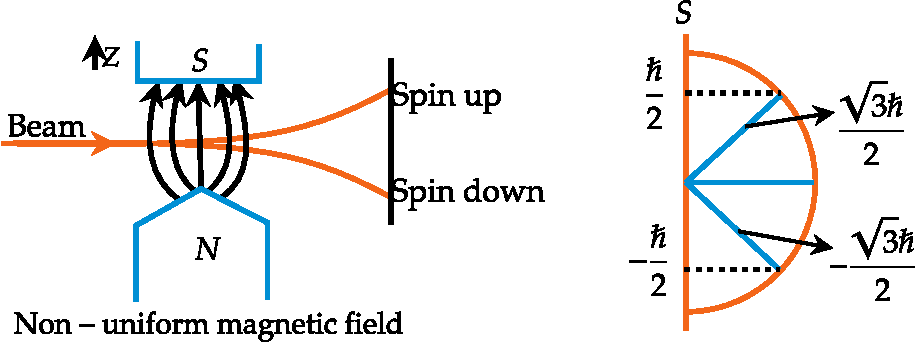
\includegraphics[height=3.5cm,width=10cm]{diagram-20220120(33)-crop}
	\caption{}
	\label{}
\end{figure}
If a beam of silver atoms passes through an in homogeneous (non-uniform) magnetic field (along z-direction), we would expect the following results:\\\\
(i) Classically, there will be a continuous band on the screen and the band will be symmetric about theundeflected direction $\mathrm{z}=0$.\\\\
(ii) Accordinh to Schrodinger's wave theory, if the atom has an orbital angular momentum ' $l$ ' then the beam will split into discrete $(2 l+1)$ components. Since, the silver atom is in ground state $(l=0)$, there will be only spot on the screen.
But, in experiments the beam splits into two distinct components.\\\\
To solve this problem, Goudsmith and Unlenbeck postulated that in addition to its orbital angular momentum the electron possesses an intrinsic angular momentum. This angular momentum has no connection with the spaial degrees of freedom but it can be related with the internal rotational or spinning mation of the electron about its own axis. This is known as spin angular momentum which is connected with an intrinsic degree of freedom i.e. spin. Spin is a purely quantum mechanical concept with classical analog. Unlike orbital angular momentum, the spin cannot be described by a differential operator.
Consider a particle of mass 'm' and charge ' $q$ ' is moving in a circle of radius ' $r$ '. The magnetic dipole moment due to the orbital motion of the particle will be
\begin{align*}
\vec{\mu}_{L}&=\frac{q}{2 m} \vec{L}
\intertext{where $\vec{L}$ is the orbital angular momentum of the particle and z-components of magnetic moment will be}
\mu_{z}&=\frac{q}{2 m} L_{z}\\
\text{For an electron the relation will be $\mu_{z}$}&=\text{$-\frac{e}{2 m_{e}} L_{z}$}\\
\text{If the electron is the eigenstates of $\hat{L}_{z}$,}&\text{ then}\\
\left(\mu_{L}\right)_{z}&=-\left(\frac{e}{2 m_{e}}\right) m_{l} \hbar=-\mu_{B} m_{l}\\
\text{where $\left(\frac{e \hbar}{2 m_{e}}\right)$ $\mu_{B}=$ Bohr magneton }&\text{and $m_{l}$ is the orbital magnetic quantum number.}\\
\text { for a particular value of } \ell, \text { we will get }(2 \ell+1) &\text { values of ' } m_{ \ell} \text { ' i.e } m_{ \ell}=- \ell,- \ell+1, \ldots \ldots  \ldots, 0,  \ldots,  \ell-1,  \ell
\intertext{Similarly, if we take electron as spinning charged sphere, then the magnetic dipole moment due to the motion of the particle will be}
\vec{\mu}_{S}&=-g_{s} \frac{e}{2 m} \vec{S}
\intertext{where $\vec{S}$ is the spin angular momentum of the electron and $g_{S}$ is the spin g-iactor. Therefore, $z$-components of magnetic dipole moment will be}
\left(\mu_{S}\right)_{z}&=-g_{S} \frac{e}{2 m} S_{z}\\
\text{If the electron is in an }&\text{eigenstate of $S_{z}$, then}\\
\text{If the electron is in an }&\text{eigenstate of $S_{z}$, then}\\
\left(\mu_{S}\right)_{z}&=-g_{s} \mu_{B} m_{s}
\end{align*}
where $\left(\frac{e \hbar}{2 m_{e}}\right)=\mu_{B}=$ Bohr magneton and $m_{s}$ is the spin magnetic quantum number.\\
For a particular value of $s$, we will get $(2 s+1)$ values of ' $m$ ' i.e. $m_{s}=-s,-s+1, \ldots \ldots ., 0, \ldots \ldots . . s-1, s$ Every fundamental particle has a specific spin $(s=0,1,2, \ldots \ldots \ldots \ldots \ldots \ldots)$\\
Fermions: Particle having half-integer spins. Examples: quarks, electrons, protons, neutrons etc.\\
 Bosons: Particles having integer spins. Example: Photons, pions, gravitons etc.\\
 Therefore, there are two kinds of angular momentum of the particle i.e.\\
 (i) Orbital angular momentum $(\vec{L})$ due to particle's orbital motion and it is characterized by two quantro numbers i.e. $\ell$ and its projection of z-axis ' $m_{\ell}$ ' which can take values from $-\ell$ to $+\ell$.\\
 (ii) Spin angular momentum $(\vec{S})$ due to some intrinsic motion of the particle and it is characterised by two quantum numbers i.e. $s$ and its projection on z-axis $m_{s}$ ' which can take values from $-s$ to $+s$. Thus, the total angular momentum can be written as
 $$ \vec{J}=\vec{L}+\vec{S} $$ and it is characterised by two quantum numbers i.e. $j$ and its projection on z-axis i.e. ' $m_{j}$ ' which can take values from $-j$ to $+j$.\\
 In the Stern-Gerlach experiment, the silver atom has orbital angular momentum to be zero i.e $l=0$ but spin angular momentum to be $1 / 2$ i.e. $s=1 / 2$. Therefore, total angular momentum will be
 $$
 j=|l-s| \text { to }|l+s|=-\frac{1}{2}, \frac{1}{2}
 $$
 For thiis, we are getting two spots on the screen.\\
 \subsection{ spin angular momentum}
 \begin{itemize}
 	\item Spin angular momentum has components $S_x,S_y,S_z$ and the corresponding operators satisfy the following commutation relation:
 	$$
 	\left[\hat{S}_{x}, \hat{S}_{y}\right]=i h \hat{S}_{z} \quad\left[\hat{S}_{y}, \hat{S}_{z}\right]=i \hbar \hat{S}_{x} \quad\left[\hat{S}_{z}, \hat{S}_{x}\right]=i \hbar \hat{S}_{y}
 	$$
 	\item $\left[\hat{S}^{2}, \hat{S}_{z}\right]=0$ i.e. they have simultaneous eigenstate as following:
 	$$
 	\begin{aligned}
 	&\hat{S}^{2}\left|s, m_{s}\right\rangle=s(s+1) \hbar^{2}\left|s, m_{s}\right\rangle \\
 	&\hat{S}_{z}\left|s, m_{s}\right\rangle=m_{s} \hbar\left|s, m_{s}\right\rangle
 	\end{aligned}
 	$$
 	\item Raising and lowering operators are defined as following:
 	$$
 	\begin{aligned}
 	&\hat{S}_{\pm}=\hat{S}_{x} \pm i \hat{S}_{y} \\
 	&\hat{S}_{+}\left|s, m_{s}\right\rangle=\hbar \sqrt{\left(s-m_{s}\right)\left(s+m_{s}+1\right)}\left|s, m_{s}+1\right\rangle \\
 	&\hat{S}_{-}\left|s, m_{s}\right\rangle=\hbar \sqrt{\left(s+m_{s}\right)\left(s-m_{s}+1\right)}\left|s, m_{s}-1\right\rangle
 	\end{aligned}
 	$$
 	\item - For a spin $\frac{1}{2}$ particles like electrons, $m_{s}$ can take values $\frac{1}{2}$ and $-\frac{1}{2}$, so the possible spin states are\\
 	Spin-up state: $\chi_{1 / 2}=|\uparrow\rangle=\left|\frac{1}{2}, \frac{1}{2}\right\rangle$\\
 	Spin-down state: $\chi_{-1 / 2}=|\downarrow\rangle=\left|\frac{1}{2},-\frac{1}{2}\right\rangle$
 	such that
 	$$\begin{aligned}
 		&\hat{S}^{2} \chi_{1 / 2}=\frac{3}{4} \hbar^{2} \chi_{1 / 2}, \quad \hat{S}^{2} \chi_{-1 / 2}=\frac{3}{4} \hbar^{2} \chi_{-1 / 2} \\
 		&\hat{S}_{z} \chi_{1 / 2}=\frac{\hbar}{2} \chi_{1 / 2}, \quad \hat{S}_{z} \chi_{-1 / 2}=\frac{\hbar}{2} \chi_{-1 / 2} \\
 		&\hat{S}_{+} \chi_{1 / 2}=0, \quad \hat{S}_{+} \chi_{-1 / 2}=\hbar \chi_{1 / 2} \\
 		&\hat{S}_{-} \chi_{1 / 2}=\hbar \chi_{-1 / 2}, \quad \hat{S}_{-} \chi_{-1 / 2}=0
 	\end{aligned}$$
 \end{itemize}
\textbf{ Matrix representation of the various spin operators for a spin-1/2 particle:}\\\\
$\hat{S}^{2}=\left[\begin{array}{ll}
	\left\langle\frac{1}{2}, \frac{1}{2}\left|\hat{S}^{2}\right| \frac{1}{2}, \frac{1}{2}\right\rangle & \left\langle\frac{1}{2}, \frac{1}{2}\left|\hat{S}^{2}\right| \frac{1}{2},-\frac{1}{2}\right\rangle \\
	\left\langle\frac{1}{2},-\frac{1}{2}\left|\hat{S}^{2}\right| \frac{1}{2}, \frac{1}{2}\right\rangle & \left\langle\frac{1}{2},-\frac{1}{2}\left|\hat{S}^{2}\right| \frac{1}{2},-\frac{1}{2}\right\rangle
\end{array}\right]=\frac{3}{4} \hbar^{2}\left[\begin{array}{ll}
	1 & 0 \\
	0 & 1
\end{array}\right]$\\\\

$\hat{S}_{z}=\left[\begin{array}{ll}
	\left\langle\frac{1}{2}, \frac{1}{2}\left|\hat{S}_{z}\right| \frac{1}{2}, \frac{1}{2}\right\rangle & \left\langle\frac{1}{2}, \frac{1}{2}\left|\hat{S}_{z}\right| \frac{1}{2},-\frac{1}{2}\right\rangle \\
	\left\langle\frac{1}{2},-\frac{1}{2}\left|\hat{S}_{z}\right| \frac{1}{2}, \frac{1}{2}\right\rangle & \left\langle\frac{1}{2},-\frac{1}{2}\left|\hat{S}_{z}\right| \frac{1}{2},-\frac{1}{2}\right\rangle
\end{array}\right]=\frac{\hbar}{2}\left[\begin{array}{cc}
	1 & 0 \\
	0 & -1
\end{array}\right]$\\\\

$\hat{S}_{+}=\left[\begin{array}{cc}
	\left\langle\frac{1}{2}, \frac{1}{2}\left|\hat{S}_{+}\right| \frac{1}{2}, \frac{1}{2}\right\rangle & \left\langle\frac{1}{2}, \frac{1}{2}\left|\hat{S}_{+}\right| \frac{1}{2},-\frac{1}{2}\right\rangle \\
	\left\langle\frac{1}{2},-\frac{1}{2}\left|\hat{S}_{+}\right| \frac{1}{2}, \frac{1}{2}\right\rangle & \left\langle\frac{1}{2},-\frac{1}{2}\left|\hat{S}_{+}\right| \frac{1}{2},-\frac{1}{2}\right\rangle
\end{array}\right]=\left[\begin{array}{ll}
	0 & \hbar \\
	0 & 0
\end{array}\right]=\hbar\left[\begin{array}{ll}
	0 & 1 \\
	0 & 0
\end{array}\right]$\\\\

$\hat{S}_{-}=\left[\begin{array}{lll}
	\left\langle\frac{1}{2}, \frac{1}{2}\left|\hat{S}_{-}\right| \frac{1}{2}, \frac{1}{2}\right\rangle & \left\langle\frac{1}{2}, \frac{1}{2}\left|\hat{S}_{-}\right| \frac{1}{2},-\frac{1}{2}\right\rangle \\
	\left\langle\frac{1}{2},-\frac{1}{2}\left|\hat{S}_{-}\right| \frac{1}{2}, \frac{1}{2}\right\rangle & \left\langle\frac{1}{2},-\frac{1}{2}\left|\hat{S}_{-}\right| \frac{1}{2},-\frac{1}{2}\right\rangle
\end{array}\right]=\hbar\left[\begin{array}{ll}
	0 & 0 \\
	1 & 0
\end{array}\right]$\\\\

$$\begin{aligned}
	&\hat{S}_{x}=\frac{1}{2}\left[\hat{S}_{+}+\hat{S}_{-}\right]=\frac{\hbar}{2}\left[\begin{array}{ll}
		0 & 1 \\
		1 & 0
	\end{array}\right] \\
	&\hat{S}_{y}=\frac{1}{2 i}\left[\hat{S}_{+}-\hat{S}_{-}\right]=\frac{\hbar}{2}\left[\begin{array}{ll}
		0 & -i \\
		i & 0
	\end{array}\right]
\end{aligned}$$
\textbf{ Eigenvalues and eigenvectors of  $\hat{S}_{z}$:}
\begin{align*}
\text{Eigenvalues: }\lambda&=\pm \frac{\hbar}{2}\\
\text{Eigenvectors: }\chi_{1 / 2}&=\left[\begin{array}{l}1 \\ 0\end{array}\right]\text{ for } \lambda=\frac{\hbar}{2}\text{ and }\chi_{-1 / 2}=\left[\begin{array}{c}0 \\ 1\end{array}\right]\text{ for }\lambda=-\frac{\hbar}{2}
\end{align*}
\textbf{$\text { Eigenvalues and eigenvectors of } \hat{S}_{x}$:}
\begin{align*}
\text{Eigenvalues: }\lambda&=\pm \frac{\hbar}{2}\\
\text{Eigenvectors: }\frac{1}{\sqrt{2}}\left[\begin{array}{l}1 \\ 1\end{array}\right]&=\frac{1}{\sqrt{2}}\left[\chi_{1 / 2}+\chi_{-1 / 2}\right]\text{ for } \lambda=\frac{\hbar}{2}\\
\text{ and }\frac{1}{\sqrt{2}}\left[\begin{array}{l}1  -1\end{array}\right]&=\frac{1}{\sqrt{2}}\left[\chi_{1 / 2}-\chi_{-1 / 2}\right]\text{ for } \lambda=-\frac{\hbar}{2}
\end{align*}
\textbf{$\text { Eigenvalues and eigenvectors of } \hat{S}_{y}$:}
\begin{align*}
\text{Eigenvalues: }\lambda&=\pm \frac{\hbar}{2}\\
\text{Eigenvectors: }\frac{1}{\sqrt{2}}\left[\begin{array}{l}1 \\ i\end{array}\right]&=\frac{1}{\sqrt{2}}\left[\chi_{1 / 2}+i \chi_{-1 / 2}\right] \text{ for }\lambda=\frac{\hbar}{2}\\
\text{ and }\frac{1}{\sqrt{2}}\left[\begin{array}{l}1 \\ -i\end{array}\right]&=\frac{1}{\sqrt{2}}\left[\chi_{1 / 2}-i \chi_{-1 / 2}\right] \text{for }\lambda=-\frac{\hbar}{2}
\end{align*}




\subsection{Pauli spin matrices}
Spin angular momentum can be related with Pauli spin vector as follows:
$$
\vec{S}=\frac{\hbar}{2} \vec{\sigma}
$$
where $\sigma_{x}=\left(\begin{array}{ll}0 & 1 \\ 1 & 0\end{array}\right), \sigma_{y}=\left(\begin{array}{cc}0 & -i \\ i & 0\end{array}\right), \sigma_{z}=\left(\begin{array}{cc}1 & 0 \\ 0 & -1\end{array}\right)$ are components of the Pauli spin vectors and known as Pauli spin matrices. These matrices satisfies the following conditions:
\begin{enumerate}[label=\roman*)]
	\item  $\sigma_{x}^{2}=\sigma_{y}^{2}=\sigma_{z}^{2}=I$
	\item  $\sigma_{j} \sigma_{k}+\sigma_{k} \sigma_{j}=\left\{\sigma_{j}, \sigma_{k}\right\}=2 I \delta_{j k}$
	\item $\left[\sigma_{j}, \sigma_{k}\right]=2 i \varepsilon_{j k l} \sigma_{l}$
	\item  Pauli spin matrices are hermitian, traceless and determinant is$-1 $
	\item  $\sigma_{x} \sigma_{y} \sigma_{z}=i I$
	\item  Since spin does not depend on spatial degrees of freedom then the components of spin $S_{x}, S_{y}, S_{z}$ commute with all spatial operators i.e. momentum, position, orbital angular momentum.
	\item $ e^{i \alpha \sigma_{j}}=I \cos \alpha+i \sigma_{j} \sin \alpha$
	\item  For any two vectors $ \vec{A} \text { and } \vec{B},(\vec{\sigma} \cdot \vec{A})(\vec{\sigma} \cdot \vec{B})=(\vec{A} \cdot \vec{B}) I+i \sigma \cdot(\vec{A} \times \vec{B})$
\end{enumerate}
\section{Addition of Angular Momenta}
Let $J_1$ and $J_2$ be two independent commuting angularmomenta vectors ie.
$$[J_1,J_2]=0$$
For example $J_1$ may be the orbital angular momentum $L$ and $J_2$ the spin $S$ of the same particle. Basis for the system is the set of simultaneous eigen states $|j_1 m_1;j_2 m_2>$ of the four commuting operators $J_1^2,J_1z,J_2^2,J_2z$ which form a complete commuting set of observables. Let us consider the set of $(2j,+1)\  (2j_2+11)$ states for fixed $j_1$ and $j_2(m_1=j_1, j_1 -1.......-j_1;m_2=j_2, j_2-1,....-j_2)$. So we suppress the fixed values of $j_1$ and $j_2$ from the notation for the basis state and write simple $|j_1 m_1 ; j_2 m_2>$ leaving it to be understood that
$$ J_1^2\ |m_1;m_2>=j_1 (j_1+1)\hbar^2 |m_1 ; m_2>$$
$$ J_2^2\ |m_1;m_2>=j_2 (j_2+1)\hbar^2 |m_1 ; m_2>$$
For $J_z$\\
$$J_1z|m_1;m_2>=m_1\hbar|m_1;m_2>,J_2z|m_1;m_2>=m_2\hbar|m_1;m_2>$$
Noting that $J_{1\pm}$ are ladder operators on $m_1$ and $J_2\pm$ on $m_2,$ Then
$$J_{1\pm}|m_1;m_2>=[(j_1\mp m_1)(j_1\pm m_1+1)]^\frac{1}{2}|m_1\pm 1;m_2>$$
$$J_{2\pm}|m_1;m_2>=[(j_2\mp m_2)(j_2\pm m_2+1)]^\frac{1}{2}|m_1;m_2\pm 1>$$
Suppose the interaction between the two system is such as to couple $J_1$ and $J_2$ then $J_1z$ and $J_2z$ are no longer constant of motion. It would be more advantageous to use other operators which commute with such an interactions for defining a basis. It is natural to use for this prupose $J^2$ and $J_z$ where $J$ is the total angular momentum operator for the composite system made up of $J_1$ and $J_2$.
$$ J=J_1+J_2\quad J^2=J_1^2+J_2^2+2J_1J_2$$
$J_1^2$ and $J_2^2$ do commute with $J^2$ and $J_z$, the simultaneous eigen state of these four operators will be taken as a new basis. We denote these by $|jm>$ is the abbreviation for $|j_1j_2j_m>$. The quantum numbers $j,m$ are of course defined by
$$ J^2|jm>=j(j+1)\hbar^2|jm>\quad J_z|jm>=m\hbar|jm>$$
\par The possible vlue of $j$ for the composite system can be obtained by stating in terms of the vector model. If $J_1$ and $J_2$ thought of as two ordinary vectors of length $j_1$ and $j_2$ respectively, these vector together with $J_1+J_2$ form a triangle. The values of $j_1, j_2, j$ must be then such that a triangle with these sides can be constructed.
\begin{figure}[H]
	\centering
	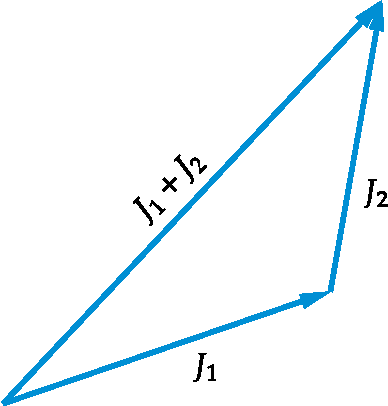
\includegraphics[height=3.5cm,width=4.5cm]{Q-2}
\end{figure}
This triangle rule or triangle condition immedietly set the maximum and minimum limits for $j$ as $(j_1+j_2)$ and $|j_1-j_2|$ (corresponding $J_1$ and $J_2$ are being parallel and antiparallel raspectively). Since angular momentum is quandized, the only allowed values between these limits are $j_1+j_2-1, j_1+j_2-2....|j_1-j_2|+1$\\
We shall now see that the same conclusion follow from quantum mechanics.\\
\par The states $|jm>$ and the sets $|m_1;m_2>$ are simple different bases for the same space. So any $|jm>$ can be written as a linear combination of the states $|m_;m_2>$
$$ |jm>=\sum_{m_1m_2}|m_1;m_2><m_1;m_2|jm>$$
The matrix formed by the elements $<m_1;m_2|jm>$ where in $m_1,m_2$ together label the rows and $j,m$ label the columns, must be unitary.\\\\
Since $J_z=J_1z+J_2z$ it is evident that 
$$m=m_1+m_2$$
ie $<m_1;m_2|jm>=0$ unless $m_2=m-m_1$\\\\
Then $|jm>$ reduces to a single sum.
$$ |jm>=\sum_{m_1}|m_1;m-m_1><m_1;m-m_1|jm>$$
Since the maximum value of $m_1$ and $m_2$ are $j_1$ and $j_2$ which is then necessarly the maximum value of $j$ too. Since this value of $m $  occurs only once (when $m_1=j_1$ and $m_2=j_2$), $j_1+j_2$ occurs only once.\\\\
Consider now the next lower value of $m$ namely $m=j_1+j_2-1$ There are two states with this $m$ one has $m_1=j_1,m_2=j_2-1$ and the other $m-1=j_1-1, m_2=j_2$ one of these or rather a linear combination of these must belongs to the value $j=j_1+j_2$ already found, since one state with each value of $m$ from $j_1+j_2$ down to $-(j_1+j_2)$ must go with this $j$\\\\
We have other state with $m=j_1+j_2-1$ which must belong to a new value of $J,j=j_1+j_2-1$\\\\
By extending this procedure $m=j_1+j_2-2$ and so on we find new values $j_1+j_2-2$ for $j$\\\\
This process ends when all the available states are exhausted. The total number of independent states is $(2j_1+1)(2j_2+1)$ as observed at the begining of this section on the other hand each value of $j$ has $2j+1$ states associated with it\\\\
So the minimum value of $j_{min}$ of $j$ is reached when 
$$ \sum_{j=J_{min}}^{j_1+j_2}(2j+1)=(2j+1)(2j_2+1)$$
After the summation of left had side we ger $J_{min}$ as $J_{min}=|j_1-j_2|$ as expected.\\
To sum up, the possible values $j$ of the total angular momentum,, resulting from the addition of two given angular momenta $j_1,j_2$ are.
$$(j_1+j_2)(j_1+j_2-1),....,|j_1-j_2|$$
\newpage 
\begin{abox}
	Practice set 1
	\end{abox}
\begin{enumerate}
	\begin{minipage}{\textwidth}
	\item The Hamiltonian of an electron in a constant magnetic field $\vec{B}$ is given by $H=\mu \vec{\sigma} \cdot \vec{B}$. where $\mu$ is a positive constant and $\vec{\sigma}=\left(\sigma_{1}, \sigma_{2}, \sigma_{3}\right)$ denotes the Pauli matrices. Let $\omega=\mu B / \hbar$ and $I$ be the $2 \times 2$ unit matrix. Then the operator $e^{i H t / \hbar}$ simplifies to
	\exyear{NET JUNE 2011}
\end{minipage}
\begin{tasks}(2)
	\task[\textbf{A.}] $I \cos \frac{\omega t}{2}+\frac{i \vec{\sigma} \cdot \vec{B}}{B} \sin \frac{\omega t}{2}$
	\task[\textbf{B.}]$I \cos \omega t+\frac{i \vec{\sigma} \cdot \vec{B}}{B} \sin \omega t$
	\task[\textbf{C.}]$I \sin \omega t+\frac{i \vec{\sigma} \cdot \vec{B}}{B} \cos \omega t$
	\task[\textbf{D.}]$I \sin 2 \omega t+\frac{i \vec{\sigma} \cdot \vec{B}}{B} \cos 2 \omega t$
\end{tasks}
\begin{minipage}{\textwidth}
	\item  In a system consisting of two spin $\frac{1}{2}$ particles labeled 1 and 2, let $\vec{S}^{(1)}=\frac{\hbar}{2} \vec{\sigma}^{(1)}$ and $\vec{S}^{(2)}=\frac{\hbar}{2} \vec{\sigma}^{(2)}$ denote the corresponding spin operators. Here $\vec{\sigma} \equiv\left(\sigma_{x}, \sigma_{y}, \sigma_{z}\right)$ and $\sigma_{x}, \sigma_{y}, \sigma_{z}$ are the three Pauli matrices.\\
	$\text { In the standard basis the matrices for the operators } S_{x}^{(1)} S_{y}^{(2)} \text { and } S_{y}^{(1)} S_{x}^{(2)} \text { are respectively, }$
	\exyear{NET JUNE 2011}
\end{minipage}
\begin{tasks}(1)
	\task[\textbf{A.}]$\frac{\hbar^{2}}{4}\left(\begin{array}{cc}
	1 & 0 \\
	0 & -1
	\end{array}\right), \frac{\hbar^{2}}{4}\left(\begin{array}{rr}
	-1 & 0 \\
	0 & 1
	\end{array}\right)$
	\task[\textbf{B.}]$\frac{\hbar^{2}}{4}\left(\begin{array}{cc}
	i & 0 \\
	0 & -i
	\end{array}\right), \frac{\hbar^{2}}{4}\left(\begin{array}{rr}
	-i & 0 \\
	0 & i
	\end{array}\right)$
	\task[\textbf{C.}]$\frac{\hbar^{2}}{4}\left(\begin{array}{cccc}
	0 & 0 & 0 & -i \\
	0 & 0 & i & 0 \\
	0 & -i & 0 & 0 \\
	i & 0 & 0 & 0
	\end{array}\right), \frac{\hbar^{2}}{4}\left(\begin{array}{cccc}
	0 & 0 & 0 & -i \\
	0 & 0 & -i & 0 \\
	0 & i & 0 & 0 \\
	i & 0 & 0 & 0
	\end{array}\right)$
	\task[\textbf{D.}]$\frac{\hbar^{2}}{4}\left(\begin{array}{cccc}
	0 & 1 & 0 & 0 \\
	1 & 0 & 0 & 0 \\
	0 & 0 & 0 & -i \\
	0 & 0 & i & 0
	\end{array}\right), \frac{\hbar^{2}}{4}\left(\begin{array}{cccc}
	0 & -i & 0 & 0 \\
	i & 0 & 0 & 0 \\
	0 & 0 & 0 & 1 \\
	0 & 0 & 1 & 0
	\end{array}\right)$
\end{tasks}
\begin{minipage}{\textwidth}
	\item $\text { These two operators of above QUESTION satisfy the relation }$
	\exyear{NET JUNE 2011}
\end{minipage}
\begin{tasks}(2)
	\task[\textbf{A.}] $\left\{S_{x}^{(1)} S_{y}^{(2)}, S_{y}^{(1)} S_{x}^{(2)}\right\}=S_{z}^{(1)} S_{z}^{(2)}$
	\task[\textbf{B.}]$\left\{S_{x}^{(1)} S_{y}^{(2)}, S_{y}^{(1)} S_{x}^{(2)}\right\}=0$
	\task[\textbf{C.}]$\left[S_{x}^{(1)} S_{y}^{(2)}, S_{y}^{(1)} S_{x}^{(2)}\right]=i S_{z}^{(1)} S_{z}^{(2)}$
	\task[\textbf{D.}] $\left[S_{x}^{(1)} S_{y}^{(2)}, S_{y}^{(1)} S_{x}^{(2)}\right]=0$
\end{tasks}
\begin{minipage}{\textwidth}
	\item The component along an arbitrary direction $\hat{n}$, with direction $\operatorname{cosines}\left(n_{x}, n_{y}, n_{z}\right)$, of the spin of a spin $-\frac{1}{2}$ particle is measured. The result is
	\exyear{NET JUNE 2012}
\end{minipage}
\begin{tasks}(2)
	\task[\textbf{A.}] 0
	\task[\textbf{B.}]$\pm \frac{\hbar}{2} n_{z}$
	\task[\textbf{C.}]$\pm \frac{\hbar}{2}\left(n_{x}+n_{y}+n_{z}\right)$
	\task[\textbf{D.}]$\pm \frac{\hbar}{2}$
\end{tasks}
\begin{minipage}{\textwidth}
	\item In a basis in which the $z$ - component $S_{z}$ of the spin is diagonal, an electron is in a spin state $\psi=\left(\begin{array}{c}(1+i) / \sqrt{6} \\ \sqrt{2 / 3}\end{array}\right) .$ The probabilities that a measurement of $S_{2}$ will yield the values $\hbar / 2$ and $-\hbar / 2$ are, respectively,
	\exyear{NET JUNE 2013}
\end{minipage}
\begin{tasks}(2)
	\task[\textbf{A.}] $1 / 2$ and $1 / 2$
	\task[\textbf{B.}]$2 / 3$ and $1 / 3$
	\task[\textbf{C.}]$1 / 4$ and $3 / 4$
	\task[\textbf{D.}]$1 / 3$ and $2 / 3$
\end{tasks}
\begin{minipage}{\textwidth}
	\item A spin $-\frac{1}{2}$ particle is in the state $\chi=\frac{1}{\sqrt{11}}\left(\begin{array}{c}1+i \\ 3\end{array}\right)$ in the eigenbasis of $S^{2}$ and $S_{2}$. If we measure $S_{z}$, the probabilities of getting $+\frac{h}{2}$ and $-\frac{h}{2}$, respectively are
	\exyear{NET DEC 2013}
\end{minipage}
\begin{tasks}(2)
	\task[\textbf{A.}] $\frac{1}{2}$ and $\frac{1}{2}$
	\task[\textbf{B.}]$\frac{2}{11}$ and $\frac{9}{11}$
	\task[\textbf{C.}] 0 and 1
	\task[\textbf{D.}]$\frac{1}{11}$ and $\frac{3}{11}$
\end{tasks}
\begin{minipage}{\textwidth}
	\item Let $\vec{\sigma}=\left(\sigma_{1}, \sigma_{2}, \sigma_{3}\right)$, where $\sigma_{1}, \sigma_{2}, \sigma_{3}$ are the Pauli matrices. If $\vec{a}$ and $\vec{b}$ are two arbitrary constant vectors in three dimensions, the commutator $[\vec{a} \cdot \vec{\sigma}, \vec{b} \cdot \vec{\sigma}]$ is equal to (in the following $I$ is the identity matrix)
	\exyear{NET DEC 2014}
\end{minipage}
\begin{tasks}(2)
	\task[\textbf{A.}] $(\vec{a} \cdot \vec{b})\left(\sigma_{1}+\sigma_{2}+\sigma_{3}\right)$
	\task[\textbf{B.}]$2 i(\vec{a} \times \vec{b}) \cdot \vec{\sigma}$
	\task[\textbf{C.}]$(\vec{a} \cdot \vec{b}) I$
	\task[\textbf{D.}]$|\vec{a}||\vec{b}| I$
\end{tasks}
\begin{minipage}{\textwidth}
	\item If $L_{i}$ are the components of the angular momentum operator $\vec{L}$, then the operator $\sum_{i=1,2,3}\left[\vec{L}, L_{i}\right]$ equals
	\exyear{NET JUNE 2015}
\end{minipage}
\begin{tasks}(2)
	\task[\textbf{A.}] $\vec{L}$
	\task[\textbf{B.}]$2 \vec{L}$
	\task[\textbf{C.}]$3 \vec{L}$
	\task[\textbf{D.}]$-\vec{L}$
\end{tasks}
\begin{minipage}{\textwidth}
	\item The Hamiltonian for a spin- $\frac{1}{2}$ particle at rest is given by $H=E_{0}\left(\sigma_{z}+\alpha \sigma_{x}\right)$, where $\sigma_{x}$ and $\sigma_{z}$ are Pauli spin matrices and $E_{0}$ and $\alpha$ are constants. The eigenvalues of this Hamiltonian are
	\exyear{NET DEC 2015}
\end{minipage}
\begin{tasks}(2)
	\task[\textbf{A.}] $\pm E_{0} \sqrt{1+\alpha^{2}}$
	\task[\textbf{B.}]$\pm E_{0} \sqrt{1-\alpha^{2}}$
	\task[\textbf{C.}]$E_{0}$ (doubly degenerate)
	\task[\textbf{D.}]$E_{0}\left(1 \pm \frac{1}{2} \alpha^{2}\right)$
\end{tasks}
\begin{minipage}{\textwidth}
	\item If $\hat{L}_{x}, \hat{L}_{y}, \hat{L}_{z}$ are the components of the angular momentum operator in three dimensions the commutator $\left[\hat{L}_{x}, \hat{L}_{x} \hat{L}_{y} \hat{L}_{z}\right]$ may be simplified to
	\exyear{NET JUNE 2016}
\end{minipage}
\begin{tasks}(2)
	\task[\textbf{A.}] $i \hbar L_{x}\left(\hat{L}_{z}^{2}-\hat{L}_{y}^{2}\right)$
	\task[\textbf{B.}]$i \hbar \hat{L}_{z} \hat{L}_{y} \hat{L}_{x}$
	\task[\textbf{C.}] $i \hbar L_{x}\left(2 \hat{L}_{z}^{2}-\hat{L}_{y}^{2}\right)$
	\task[\textbf{D.}]0
\end{tasks}
\begin{minipage}{\textwidth}
	\item The Hamiltonian of a spin $\frac{1}{2}$ particle in a magnetic field $\vec{B}$ is given by $H=-\mu \cdot \vec{B} \cdot \vec{\sigma}$, where $\mu$ is a real constant and $\vec{\sigma}=\left(\sigma_{x}, \sigma_{y}, \sigma_{z}\right)$ are the Pauli spin matrices. If $\vec{B}=\left(B_{0}, B_{0}, 0\right)$ and the spin state at time $t=0$ is an eigenstate of $\sigma_{x}$, then of the expectation values $\left\langle\sigma_{x}\right\rangle,\left\langle\sigma_{y}\right\rangle$ and $\left\langle\sigma_{z}\right\rangle$
	\exyear{NET JUNE 2018}
\end{minipage}
\begin{tasks}(2)
	\task[\textbf{A.}] only $\left\langle\sigma_{x}\right\rangle$ changes with time
	\task[\textbf{B.}] only $\left\langle\sigma_{y}\right\rangle$ changes with time
	\task[\textbf{C.}]only $\left\langle\sigma_{z}\right\rangle$ changes with time
	\task[\textbf{D.}]all three change with time
\end{tasks}
\end{enumerate}

\colorlet{ocre1}{ocre!70!}
\colorlet{ocrel}{ocre!30!}
\setlength\arrayrulewidth{1pt}
\begin{table}[H]
	\centering
	\arrayrulecolor{ocre}
	
	\begin{tabular}{|p{1.5cm}|p{1.5cm}||p{1.5cm}|p{1.5cm}|}
		\hline
		\multicolumn{4}{|c|}{\textbf{Answer key}}\\\hline\hline
		\rowcolor{ocrel}Q.No.&Answer&Q.No.&Answer\\\hline
		1&\textbf{b}&2&\textbf{c}\\\hline
		3&\textbf{d}&4&\textbf{d}\\\hline
		5&\textbf{d}&6&\textbf{b}\\\hline
		7&\textbf{b}&8&\textbf{b}\\\hline
		9&\textbf{a}&10&\textbf{a}\\\hline
		11&\textbf{d}&&\\\hline
	\end{tabular}
\end{table}



\newpage 
\begin{abox}
Practice set 2 
\end{abox}
\begin{enumerate}
\begin{minipage}{\textwidth}
	\item $\text { For a spin-s particle, in the eigen basis of } \vec{S}^{2}, S_{x} \text { the expectation value }\left\langle s m\left|S_{x}^{2}\right| s m\right\rangle \text { is }$
	\exyear{GATE 2010}
\end{minipage}
\begin{tasks}(2)
	\task[\textbf{A.}] $\frac{\hbar^{2}\left\{s(s+1)-m^{2}\right\}}{2}$
	\task[\textbf{B.}] $\hbar^{2}\left\{s(s+1)-2 m^{2}\right\}$
	\task[\textbf{C.}]$\hbar^{2}\left\{s(s+1)-m^{2}\right\}$
	\task[\textbf{D.}]$\hbar^{2} m^{2}$
\end{tasks}
\begin{minipage}{\textwidth}
	\item If $L_{x}, L_{y}$ and $L_{z}$ are respectively the $x, y$ and $z$ components of angular momentum operator $L$. The commutator $\left[L_{x} L_{y}, L_{z}\right]$ is equal to
	\exyear{GATE 2011}
\end{minipage}
\begin{tasks}(2)
	\task[\textbf{A.}] $i \hbar\left(L_{x}^{2}+L_{y}^{2}\right)$
	\task[\textbf{B.}]$2 i \hbar L_{z}$
	\task[\textbf{C.}]$i \hbar\left(L_{x}^{2}-L_{y}^{2}\right)$
	\task[\textbf{D.}]0
\end{tasks}
\begin{minipage}{\textwidth}
	\item Which one of the following commutation relations is NOT CORRECT? Here, symbols have their usual meanings.
	\exyear{GATE 2013}
\end{minipage}
\begin{tasks}(2)
	\task[\textbf{A.}] $\left[L^{2}, L_{z}\right]=0$
	\task[\textbf{B.}]$\left\lfloor L_{x}, L_{y}\right\rfloor=i \hbar L_{z}$
	\task[\textbf{C.}]$\left[L_{z}, L_{+}\right]=\hbar L_{+}$
	\task[\textbf{D.}]$\left[L_{z}, L_{-}\right]=\hbar L_{-}$
\end{tasks}
\begin{minipage}{\textwidth}
	\item A spin-half particle is in a linear superposition $0.8|\uparrow\rangle+0.6|\downarrow\rangle$ of its spin-up and spindown states. If $|\uparrow\rangle$ and $|\downarrow\rangle$ are the eigenstates of $\sigma_{z}$, then what is the expectation value up to one decimal place, of the operator $10 \sigma_{z}+5 \sigma_{x}$ ? Here, symbols have their usual meanings.
	\exyear{GATE 2013}
\end{minipage}
\begin{minipage}{\textwidth}
	\item If $\vec{L}$ is the orbital angular momentum and $\bar{S}$ is the spin angular momentum, then $\vec{L} \cdot \vec{S}$ does not commute with
	\exyear{GATE 2014}
\end{minipage}
\begin{tasks}(2)
	\task[\textbf{A.}] $S_{z}$ 
	\task[\textbf{B.}]$L^{2}$
	\task[\textbf{C.}]$S^{2}$
	\task[\textbf{D.}]$(\vec{L}+\vec{S})^{2}$
\end{tasks}
\begin{minipage}{\textwidth}
	\item If $L_{+}$and $L_{-}$are the angular momentum ladder operators then the expectation value of $\left(L_{+} L_{-}+L_{-} L_{+}\right)$in the state $|l=1, m=1\rangle$ of an atom is $\hbar^{2}$
	\exyear{GATE 2014}
\end{minipage}
\begin{minipage}{\textwidth}
	\item The Pauli matrices for three spin $-\frac{1}{2}$ particles are $\vec{\sigma}_{1}, \vec{\sigma}_{2}$ and $\vec{\sigma}_{3}$, respectively. The dimension of the Hilbert space required to define an operator $\hat{O}=\vec{\sigma}_{1} \cdot \vec{\sigma}_{2} \times \vec{\sigma}_{3}$ is
	\exyear{GATE 2015}
\end{minipage}
\begin{minipage}{\textwidth}
	\item Let the Hamiltonian for two spin-1/2 particles of equal masses $m$, momenta $\vec{p}_{1}$ and $\vec{p}_{2}$ and positions $\vec{r}_{1}$ and $\vec{r}_{2}$ be $H=\frac{1}{2 m} p_{1}^{2}+\frac{1}{2 m} p_{2}^{2}+\frac{1}{2} m \omega^{2}\left(r_{1}^{2}+r_{2}^{2}\right)+k \vec{\sigma}_{1} \cdot \vec{\sigma}_{2}$, where $\vec{\sigma}_{1}$ and $\vec{\sigma}_{2}$ denote the corresponding Pauli matrices, $\hbar \omega=0.1 \mathrm{eV}$ and $k=0.2 \mathrm{eV}$. If the ground state has net spin zero, then the energy (in $\mathrm{eV}$ ) is
	\exyear{GATE 2015}
\end{minipage}
\begin{minipage}{\textwidth}
	\item If $\vec{s}_{1}$ and $\vec{s}_{2}$ are the spin operators of the two electrons of a He atom, the value o $\left\langle\vec{s}_{1} \cdot \vec{s}_{2}\right\rangle$ for the ground state is
	\exyear{GATE 2016}
\end{minipage}
\begin{tasks}(2)
	\task[\textbf{A.}] $-\frac{3}{2} \hbar^{2}$
	\task[\textbf{B.}]$-\frac{3}{4} \hbar^{2}$
	\task[\textbf{C.}] 0
	\task[\textbf{D.}] $\frac{1}{4} \hbar^{2}$
\end{tasks}
\begin{minipage}{\textwidth}
	\item The Hamiltonian of a spin $\frac{1}{2}$ particle in a magnetic field $\vec{B}$ is given by $H=-\mu \cdot \vec{B} \cdot \vec{\sigma}$, where $\mu$ is a real constant and $\vec{\sigma}=\left(\sigma_{x}, \sigma_{y}, \sigma_{z}\right)$ are the Pauli spin matrices. If $\vec{B}=\left(B_{0}, B_{0}, 0\right)$ and the spin state at time $t=0$ is an eigenstate of $\sigma_{x}$, then of the expectation values $\left\langle\sigma_{x}\right\rangle,\left\langle\sigma_{y}\right\rangle$ and $\left\langle\sigma_{z}\right\rangle$
	\exyear{NET JUNE 2018}
\end{minipage}
\begin{tasks}(2)
	\task[\textbf{A.}] only $\left\langle\sigma_{x}\right\rangle$ changes with time
	\task[\textbf{B.}] only $\left\langle\sigma_{y}\right\rangle$ changes with time
	\task[\textbf{C.}]only $\left\langle\sigma_{z}\right\rangle$ changes with time
	\task[\textbf{D.}]all three change with time
\end{tasks}
\begin{minipage}{\textwidth}
	\item For the Hamiltonian $H=a_{0} I+\vec{b} \cdot \vec{\sigma}$ where $a_{0} \in R, \vec{b}$ is a real vector, $I$ is the $2 \times 2$ identity matrix, and $\vec{\sigma}$ are the Pauli matrices, the ground state energy is
	\exyear{GATE 2017}
\end{minipage}
\begin{tasks}(2)
	\task[\textbf{A.}] $|b|$
	\task[\textbf{B.}]$2 a_{0}-|b|$
	\task[\textbf{C.}]$a_{0}-|b|$
	\task[\textbf{D.}]$a_{0}$
\end{tasks}
\end{enumerate}

\colorlet{ocre1}{ocre!70!}
\colorlet{ocrel}{ocre!30!}
\setlength\arrayrulewidth{1pt}
\begin{table}[H]
	\centering
	\arrayrulecolor{ocre}
	
	\begin{tabular}{|p{1.5cm}|p{1.5cm}||p{1.5cm}|p{1.5cm}|}
		\hline
		\multicolumn{4}{|c|}{\textbf{Answer key}}\\\hline\hline
		\rowcolor{ocrel}Q.No.&Answer&Q.No.&Answer\\\hline
		1&\textbf{a}&2&\textbf{c}\\\hline
		3&\textbf{d}&4&\textbf{7.6}\\\hline
		5&\textbf{d}&6&\textbf{2}\\\hline
		7&\textbf{8}&8&\textbf{-0.3}\\\hline
		9&\textbf{b}&10&\textbf{c}\\\hline
		11&\textbf{c}&&\\\hline
	\end{tabular}
\end{table}




\newpage
\begin{abox}
	Practice set 3
	\end{abox}
\begin{enumerate}
	\begin{minipage}{\textwidth}
	\item Two spin half particle identified as $\vec{S}_{1}$ and $\vec{S}_{2}$ and $\theta$ is angle between them. If they are in singlet configuration, then find the value of $\left\langle\vec{S}_{1} \cdot \vec{S}_{2}\right\rangle$.
\end{minipage}
\begin{answer}
	$\vec{S}=\vec{S}_{1}+\vec{S}_{2}$\\
	\begin{align*}
		&\vec{S}_{1} \cdot \vec{S}_{2}=\frac{S^{2}-S_{1}^{2}-S_{2}^{2}}{2} \\
		&\therefore S_{1}=\frac{1}{2}, S_{2}=\frac{1}{2} \Rightarrow S=0 \text { (singlet) } S=1 \text { (Triplet) } \\
		&\left\langle S_{1}^{2}\right\rangle=\frac{3}{4} \hbar^{2} \quad\left\langle S_{2}^{2}\right\rangle=\frac{3}{4} \hbar^{2} \\
		&\langle S\rangle=0 \hbar^{2}(\text { for singlet }) \therefore\left\langle\vec{S}_{1} \cdot \vec{S}_{2}\right\rangle=\frac{\langle S\rangle^{2}-\left\langle S_{1}\right\rangle^{2}-\left\langle S_{2}\right\rangle^{2}}{2}=\frac{0-\frac{3}{4} \hbar^{2}-\frac{3}{4} \hbar^{2}}{2} \cdot\\
		&\left\langle\vec{S}_{1} \cdot \vec{S}_{2}\right\rangle=\frac{-3}{4} \hbar^{2}
	\end{align*}
\end{answer}


	\begin{minipage}{\textwidth}
	\item The components of arbitrary vectors $A$ and $B$ commute with those of $\sigma$.
	Show that $(\sigma \cdot A)(\sigma \cdot B)=A \cdot B+i \sigma \cdot(A \times B)$.
\end{minipage}
\begin{answer}
	$(\sigma . A)(\sigma . B)=\left(\sigma_{x} A_{x}+\sigma_{y} A_{y}+\sigma_{z} A_{z}\right)\left(\sigma_{x} B_{x}+\sigma_{y} B_{y}+\sigma_{z} B_{z}\right)$\\\\ $=\sigma_{x}^{2} A_{x} B_{x}+\sigma_{y}^{2} A_{y} B_{y}+\sigma_{z}^{2} A_{z} B_{z}+\sigma_{x} \sigma_{y} A_{x} B_{y}+\sigma_{y} \sigma_{x} A_{y} B_{x}$\\ $\quad+\sigma_{x} \sigma_{z} A_{x} B_{z}+\sigma_{y} \sigma_{z} A_{y} B_{z}+\sigma_{z} \sigma_{y} A_{z} B_{y}+\sigma_{z} \sigma_{x} A_{z} B_{x}$\\\\
	Using the relations $\sigma_{x}^{2}=\sigma_{y}^{2}=\sigma_{z}^{2}=1, \sigma_{x} \sigma_{y}=i \sigma_{z}, \sigma_{y} \sigma_{z}=i \sigma_{x}, \sigma_{z} \sigma_{x}=i \sigma_{y}$,\\
	$\sigma_{x} \sigma_{y}+\sigma_{y} \sigma_{x}=\sigma_{y} \sigma_{z}+\sigma_{z} \sigma_{y}=\sigma_{z} \sigma_{x}+\sigma_{x} \sigma_{z}=0$\\
	$$\begin{aligned}
	\text { We get }(\sigma \cdot A)(\sigma \cdot B) &=(A \cdot B)+i \sigma_{z}\left(A_{x} B_{y}-A_{y} B_{x}\right)+i \sigma_{y}\left(A_{z} B_{x}-A_{x} B_{z}\right)+i \sigma_{x}\left(A_{y} B_{z}-A_{z} B_{y}\right) \\
	&=(A \cdot B)+i \sigma \cdot(A \times B)
	\end{aligned}$$
\end{answer}
	\begin{minipage}{\textwidth}
	\item Find the equivalence of the following operators:\\\\
	(i) $S_{x}^{2} S_{y} S_{z}^{2}$;\\\\
	(ii) $S_{x}^{2} S_{y}^{2} S_{z}^{2}$;\\\\
	(iii) $S_{x} S_{y} S_{z}^{3}$
\end{minipage}
\begin{answer}
	$\text { (i) } S_{x}^{2} S_{y} S_{z}^{2}=\left(\frac{\hbar}{2}\right)^{2} \sigma_{x}^{2} \frac{\hbar}{2} \sigma_{y}\left(\frac{\hbar}{2}\right)^{2} \sigma_{z}^{2}=\left(\frac{\hbar}{2}\right)^{5} \sigma_{y}$\\\\
	$\text { (ii) } S_{x}^{2} S_{y}^{2} S_{z}^{2}=\left(\frac{\hbar}{2}\right)^{2} \sigma_{x}^{2}\left(\frac{\hbar}{2}\right)^{2} \sigma_{y}^{2}\left(\frac{\hbar}{2}\right)^{2} \sigma_{z}^{2}=\left(\frac{\hbar}{2}\right)^{6}$\\\\
	$\text { (iii) } S_{x} S_{y} S_{z}^{3}=\frac{\hbar}{2} \sigma_{x} \frac{\hbar}{2} \sigma_{y}\left(\frac{\hbar}{2}\right)^{3} \sigma_{x}^{3}=\left(\frac{\hbar}{2}\right)^{5} \sigma_{x} \sigma_{y} \sigma_{z}=\left(\frac{\hbar}{2}\right)^{5} i$	
\end{answer}
	\begin{minipage}{\textwidth}
	\item $\vec{J}=\vec{L}+\vec{S}$ where $\vec{J}$ is total angular momentum and $\vec{L}$ and $\vec{S}$ are orbital angl momentum and spin angular momentum respectively. Find the value of $a<L . S>$.
\end{minipage}
\begin{answer}
	$J=L+S$
	$$
	\begin{aligned}
	J^{2} &=(L+S)(L+S)=L^{2}+L \cdot S+S \cdot L+S^{2} \\
	&=L^{2}+S^{2}+2 L \cdot S \quad \because S \cdot L=L \cdot S \\
	L \cdot S &=\frac{1}{2}\left(J^{2}-L^{2}-S^{2}\right) \Rightarrow\langle L \cdot S\rangle=\frac{\hbar^{2}}{2}\left[j(j+1)-l(l+1)-s(s+1)\right]
	\end{aligned}
	$$	
\end{answer}
	\begin{minipage}{\textwidth}
	\item Find the energy level of spin $s=1 / 2$ particle whose Hamiltonion is given by
	$$
	\hat{H}=\frac{\alpha}{\hbar^{2}}\left(S_{x}^{2}+S_{y}^{2}-2 S_{z}^{2}\right)-\frac{\beta}{\hbar} S_{z}
	$$
	where $\alpha$ and $\beta$ are constants. What is degeneracy of the energy?
\end{minipage}
\begin{answer}
	$\mathrm{H}=\frac{\alpha}{\hbar^{2}}\left(S_{x}^{2}+S_{y}^{2}-2 S_{z}^{2}\right)-\frac{\beta}{\hbar} S_{z} \Rightarrow S^{2}=S_{x}^{2}+S_{y}^{2}+S_{z}^{2}, S_{x}^{2}+S_{y}^{2}=S^{2}-S_{z}^{2}$ \\
	$\Rightarrow H=\frac{\alpha}{\hbar^{2}}\left(S^{2}-S_{z}^{2}-2 S_{z}^{2}\right)-\frac{\beta}{\hbar} S_{z}$\\
	$=\frac{\alpha}{\hbar^{2}}\left(S^{2}-3 S_{z}^{2}\right)-\frac{\beta}{\hbar} S_{z}=\frac{\alpha}{\hbar^{2}}\left(s(s+1) \hbar^{2}-3 m^{2} \hbar^{2}\right)-\frac{\beta}{\hbar} m \hbar=\frac{3 \alpha}{4}-m(3 m+\beta)$ \\
	The degeneracy of the system is $(2 s+1)$ i.e. $\left[2\left(\frac{1}{2}\right)+1\right]=2$	
\end{answer}
	\begin{minipage}{\textwidth}
	\item 	Consider a system which is initially in the state
	$$
	\psi(\theta, \phi)=\frac{1}{\sqrt{5}} Y_{1,-1}(\theta, \phi)+\sqrt{\frac{3}{5}} Y_{1,0}(\theta, \phi)+\frac{1}{\sqrt{5}} Y_{1,1}(\theta, \phi)
	$$
	(i) If $L^{2}$ is measured $\psi(\theta, \phi)$ then what is the measured with what probability?\\
	(ii) If $L_{z}$ is measured $\psi(\theta, \phi)$ then what is the measured with what probability?\\
	(iii) What is the expectation value of $L^{2}$ and $L_{z}$
\end{minipage}
\begin{answer}
	(i) If $L^{2}$ measured $\psi(\theta, \phi)$ then it will measured either $Y_{1,-1}$ or $Y_{1,0}$ or $Y_{1,1}$ each time. The measurement is $l(l+1) \hbar^{2}$ i.e. $2 \hbar^{2}$ and the probability of measurement is $\left(\frac{1}{\sqrt{5}}\right)^{2}+\left(\sqrt{\frac{3}{5}}\right)^{2}+\left(\frac{1}{\sqrt{5}}\right)^{2}$ i.e. 1 .\\
	(ii) If $L_{z}$ measured on $\psi(\theta, \phi)$ then it will measured either $Y_{1,-1}$ or $Y_{1,0}$ or $Y_{1,1}$.\\
	The measurement of $L_{2}$ on $Y_{1,1}$ yields $1 \hbar$ with probability $1 / 5$.\\
	The measurement of $L_{z}$ on $Y_{1,0}$ yields $0 \hbar$ with probability $3 / 5$.\\
	The measurement of $L_{z}$ on $Y_{1,-1}$ yields $-1 \hbar$ with probability $1 / 5$.\\
	(iii) The expectation value of $L^{2}$ is given as
	$$
	2 \hbar^{2} \cdot \frac{1}{5}+2 \hbar^{2} \cdot \frac{3}{5}+2 \hbar^{2} \cdot \frac{1}{5}=2 \hbar^{2}
	$$
	The expectation value of $L_{z}$ is given as $1 \hbar \cdot \frac{1}{5}+0 \hbar \cdot \frac{3}{5}+(-1 \hbar) \cdot \frac{1}{5}=0$
\end{answer}
\end{enumerate}





